\begin{problem}
Suppose students in Princeton Astrophysics invent a new card game, whose rules we don't concern ourselves with. The cards of the game have 11 circles each, arranged with five-fold symmetry as follows:
\begin{center}
    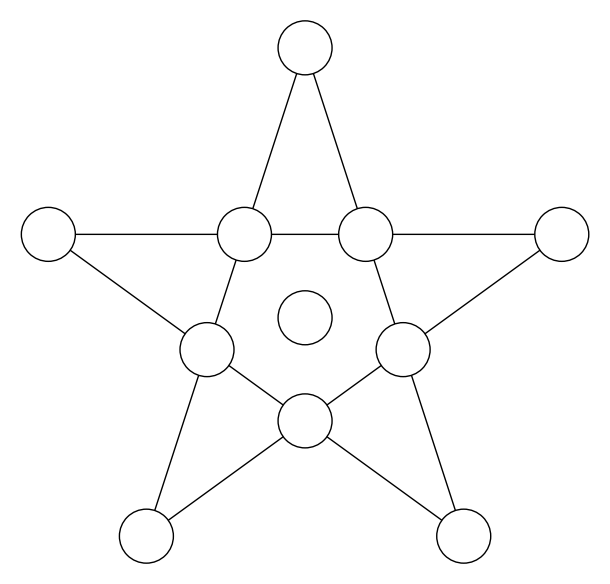
\includegraphics[width=0.4\textwidth]{image/pentagonthing.png}
\end{center}
On each card, 3 circles will be colored orange, and the remaining 8 will be colored black, in keeping with the color traditions of Princeton University. Two colorings are considered the same if and only if one can be carried to the other by a rotation or a reflection. How many different colorings are there?
\end{problem}